\documentclass[12pt,a4paper]{article}
\usepackage{fullpage}
\usepackage[margin=2cm]{geometry}
\usepackage{amsmath}
\usepackage{subfig}
\usepackage{graphicx}
\usepackage[justification=centering]{caption}
\begin{document}
\title{Improving the results from Convolutional Neural Network on pronotum images}
\author{LE Van Linh and BEURTON-AIMAR Marie}
\date{November, 2017}
\maketitle
\begin{abstract}
In the last study, we have presented a convolutional neural network (CNN) to predict the landmarks on pronotum part of Beetles. The results have shown that the network has worked well when it can be detected the landmarks on pronotum images when we considered on the side of statistic problem. However, when we displayed the coordinate of the predicted landmarks on the images, the predicted locations have still not precise, specifically, the landmarks stayed on the shape border and at the corner of pronotum. In this report, we describe a method to improve the locations of the landmarks which stay at the corner of the pronotum shape\footnote{Segmentation results} and have been predicted by CNN, i.e $3{rd}, 4^{th}, 6^{th}$ and $7^{th}$ landmark. The method uses a mean model to indicate the new location of predicted landmark (by CNN) on the curve. The effect of method is evaluated by comparing the distances from two predicted landmarks to manual landmark.
\end{abstract}

\section{The results from CNN}
In this section, we reminded the results that we have obtained from CNN. According to the results, to assess the accuracy of predicted landmark position, the distance between predicted landmark and manual landmark have been calculated. Then, the average distance of the landmarks that have the same index on all images is calculated (based on the index of the landmark). Table.\ref{avgdistance1} shows the average distance on each landmark of pronotum images:\\
\begin{table}[h!]
	\centering
	\begin{tabular}{l l l l l l l l l}
	 Landmark& LM 1 & LM 2 & \textbf{LM 3} & \textbf{LM 4} & LM 5 & \textbf{LM 6} & \textbf{LM 7} & LM 8 \\ \hline
 	 Average & 4.0020 &	4.4831 & \textbf{4.2959} & \textbf{4.3865} &	 4.2925 & \textbf{5.3631} & \textbf{4.6360} &	4.9362
 \\ \hline
	\end{tabular}
	\caption{The average distance on each landmark }
	\label{avgdistance1}
\end{table}~\\
The predicted landmark is considered as well-predicted if the distance from it is less than the average value of its index. Fig.\ref{wellpredicted} shows the proportions of well-predicted landmarks on pronotum images.
\begin{figure}[h!]
	\centering
	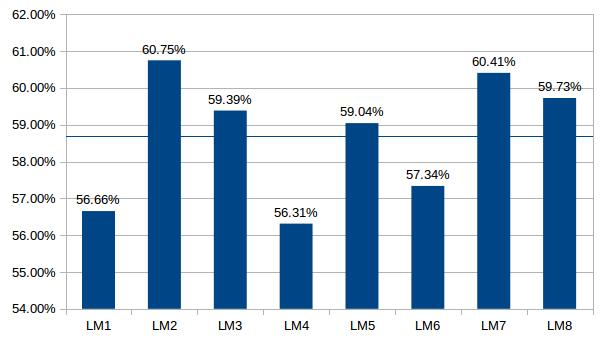
\includegraphics[scale=0.5]{images/pronotum_avg_eval}
	\caption{The proportions of well-predicted landmarks on pronotum}
	\label{wellpredicted}
\end{figure}
\section{Method}
In this section, we describe the method that used to improve the position of the landmarks which have been predicted by CNN. The landmarks are stayed on the contours of the pronotum, specific, the landmarks at position $3^{rd}, 4^{th}, 5^{th}$, and $6^{th}$. The main steps of this method include:
\begin{enumerate}
	\item Generating (choosing) the ``mean curve" at each landmark position (from manual landmark),
	\item Adapting the predicted landmark on the contour of pronotum,
	\item Searching a position around ``adapted point" that the curve via it is closest with the ``mean curve".
\end{enumerate}
\subsection*{Generating mean curve}
The mean curve is computed from a set of curves via the manual landmarks that have the same order. The inputs of this step are set of training images and their manual landmarks that have the same order. Firstly, the images are segmented. Secondly, for a segmented image and its manual landmark, a patch with the size of $7 \times 7$ is extracted centering at the manual landmark. Thirdly, the contour points that stay inside the patch are detected. At the end, the contour points are sorted and the points on the mean curve are obtained by computing the mean coordinates of corresponding contours points. Fig.\ref{meancuvre} shows the mean curve through the $3^{rd}$ and the $7^{th}$ landmarks. In the image, the 1-positions present for the points belongs to the mean curve (red paths). 
\begin{figure}[h!]
\centering
\subfloat[Mean curve of $3^{rd}$ landmark]{\label{mean_lm3}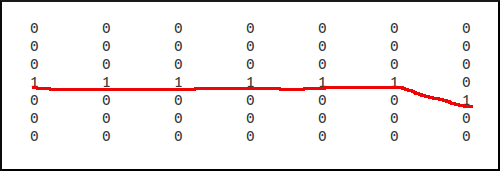
\includegraphics[width=0.5\textwidth]{./images/mean_cv_lm3}}~~
\subfloat[Mean curve of $7^{th}$ landmark]{\label{mean_lm7}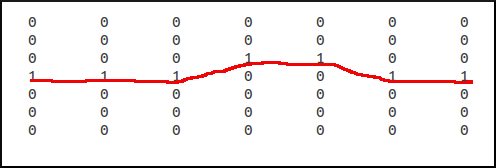
\includegraphics[width=0.5\textwidth]{./images/mean_cv_lm7}}
\caption{The mean curve through the $3^{rd}$ and $7^{th}$ landmarks}
\label{meancuvre}
\end{figure}~\\
In another approach, the user can extract the curve (in the patch) through the manual landmarks of all images. Then, choosing randomly a curve and use it as the mean curve \textit{i.e the $84^{th}$ image}.
\subsection*{Adapting the predicted landmark}
The landmark which has been predicted by CNN, has closed to the pronotum but it did not mostly stay on the curve. This step tries to adapt the predicted landmark on the curve. The point on the curve replace for the predicted-landmark has the minimum distance with it. It means that we try to find the point on the contour points that has the minimum distance to the predicted landmark.
\subsection*{Improving predicted position}
After finding the point on contour to replace the predicted landmark. A patch with the size of $15 \times 15$ is created centering at this point. For each contour point belongs to the patch, a small patch with the same size of ``mean curve" patch ($7 \times 7$) is extracted. Then, the contour points belong to the ``small patch" are used to compare with the mean curve (actually, it is also a list of points). The process finishes when all points in the patch ($15 \times 15$) are considered. New coordinates of predicted landmark are the point that has the minimum distance with the mean curve.
\section{Experiments}
The method has experimented on the $3^{rd}$ and $7^{th}$ landmarks. For each landmark, the mean curve has been generated by two ways:
\begin{enumerate}
	\item Generating from a set of image and manual landmarks (rule 1),
	\item Choosing randomly a landmark of an image (rule 2).
\end{enumerate}
During the process to find the new position of predicted-landmark, Root Mean Square Distance (RMSD) is used to compute the distance between a candidate curve and mean curve. At the end, the average distance of all new predicted landmark and its corresponding manual landmark is computed and compared with the last result (result from CNN). Table \ref{avgdistance2} shows a comparison between the average distances from predicted landmark to manual landmark.
\begin{table}[h!]
	\centering
	\begin{tabular}{l l l l }
	 Landmark & CNN & Rule 1 & Rule 2 \\ \hline
 	 $3^{rd}$ & 4.2959 & 2.8421 & 3.4255 \\ \hline
 	 $7^{th}$ & 4.6360 &	3.4166 & 3.0335 \\ \hline
	\end{tabular}
	\caption{The average distance on each landmark according to the mean curve generating rules}
	\label{avgdistance2}
\end{table}~\\
In another side, when we consider on the number of well predicted landmarks (the distance from it to corresponding manual one is less than average value), the proportions are also significantly improved. Fig. shows the proportion of well-predicted on the $3^{rd}$ and $7^{th}$ landmarks.
\begin{figure}[h!]
\centering
\subfloat[The $3^{rd}$ landmark]{\label{mean_lm3}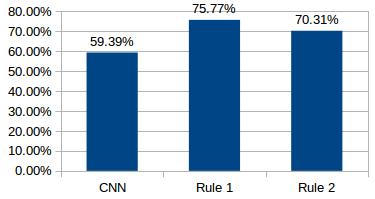
\includegraphics[width=0.5\textwidth]{./images/mean_proportions_lm3}}~~
\subfloat[The $7^{th}$ landmark]{\label{mean_lm7}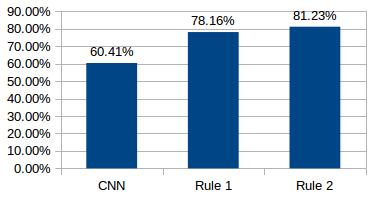
\includegraphics[width=0.5\textwidth]{./images/mean_proportions_lm7}}
\caption{The proportions of well-predicted of the $3^{rd}$ and $7^{th}$ landmarks}
\label{meancuvre}
\end{figure}~\\


\section{Conclusions}
In this study, we described a method to improve the location of the predicted landmark by CNN. The method mainly based on the segmentation technique. We extract the contour points of the pronotum; then, the mean contour through the manual landmarks are computed. At the end, we find the new position of the predicted landmark. The new position of the landmark is evaluated by computing the distance from it to manual one and comparing with the previous distance. The results are shown that the location of a number predicted landmarks have been improved. The new positions are more closest with the manual one than the landmark at the beginning.
\bibliographystyle{unsrt}
\bibliography{includes/references}
\pagebreak

\end{document}